% ------------------------------------------------------------------------------
% TYPO3 CMS 7.5 - What's New - Chapter "Introduction" (French Version)
%
% @author	Michael Schams <schams.net>
% @license	Creative Commons BY-NC-SA 3.0
% @link		http://typo3.org/download/release-notes/whats-new/
% @language	French
% ------------------------------------------------------------------------------
% LTXE-CHAPTER-UID:		3a84d600-9fb67dda-31c4af65-dd7a4af5
% LTXE-CHAPTER-NAME:	Introduction
% ------------------------------------------------------------------------------

\section{Introduction}
\begin{frame}[fragile]
	\frametitle{Introduction}

	\begin{center}\huge{Introduction}\end{center}
	\begin{center}\huge{\color{typo3darkgrey}\textbf{Faits}}\end{center}

\end{frame}

% ------------------------------------------------------------------------------
% LTXE-SLIDE-START
% LTXE-SLIDE-UID:		7e21671d-ee774188-0b062c9e-ceb3e41f
% LTXE-SLIDE-ORIGIN:	81d53787-fb3806f0-841b4042-7033fad4 English
% LTXE-SLIDE-ORIGIN:	f1ea1041-2b6b2b81-f54b45c0-84265d6a German
% LTXE-SLIDE-TITLE:		TYPO3 CMS 7.5 - The Facts
% ------------------------------------------------------------------------------
\begin{frame}[fragile]
	\frametitle{Introduction}
	\framesubtitle{TYPO3 CMS 7.5 - Faits}

	\begin{itemize}
		\item Date de sortie~: 29 Septembre 2015
		\item Type de sortie~: "Sprint Release"
		\item Slogan~: Embrace, Innovate, Deliver
		\item Axe principal~: Finalization
	\end{itemize}

	\begin{figure}
		
\includegraphics[width=0.95\linewidth]{Introduction/typo3cms75-banner.jpg}
	\end{figure}

\end{frame}

% ------------------------------------------------------------------------------
% LTXE-SLIDE-START
% LTXE-SLIDE-UID:		fa8d6d8f-cd635731-dd50c541-b9f61405
% LTXE-SLIDE-ORIGIN:	a0327db8-b4a9bd42-f32515d0-87296684 English
% LTXE-SLIDE-ORIGIN:	5d8adc7d-af29cb46-4acd2255-27362935 German
% LTXE-SLIDE-TITLE:		System Requirements
% ------------------------------------------------------------------------------
\begin{frame}[fragile]
	\frametitle{Introduction}
	\framesubtitle{Prérequis système}

	\begin{itemize}
		\item PHP*~:\tabto{3cm}v5.5.0 - v5.6.x
		\item MySQL~:\tabto{3cm}v5.5.x - v5.6.x (pas de mode strict)
		\item Espace disque~:\tabto{3cm}min. 200 Mo
		\item Configuration PHP~:

			\begin{itemize}
				\item memory\_limit >= 128M
				\item max\_execution\_time >= 240s
				\item L'option de compilation \texttt{--disable-ipv6} \underline{NE} doit \underline{PAS} être utilisée
			\end{itemize}

		\item Le backend nécessite IE >= 9 ou tout autre navigateur moderne

	\end{itemize}

	\vspace{.8cm}
	*) Plus d'information~: \href{http://typo3.org/news/article/php-minimum-requirements-for-typo3-cms-7/}{Prérequis PHP minimum pour TYPO3 CMS 7 (en anglais)}

\end{frame}

% ------------------------------------------------------------------------------
% LTXE-SLIDE-START
% LTXE-SLIDE-UID:		68ba0ff6-4120874d-cc0e2899-a7ebc799
% LTXE-SLIDE-ORIGIN:	c155d534-1a53682d-f56423dc-163111d3 English
% LTXE-SLIDE-ORIGIN:	6cad14bf-08874e74-1dd85333-e5c43a08 German
% LTXE-SLIDE-TITLE:		Development And Release Timeline
% ------------------------------------------------------------------------------
\begin{frame}[fragile]
	\frametitle{Introduction}
	\framesubtitle{Chronologie des développements et sorties}

	\begin{figure}
		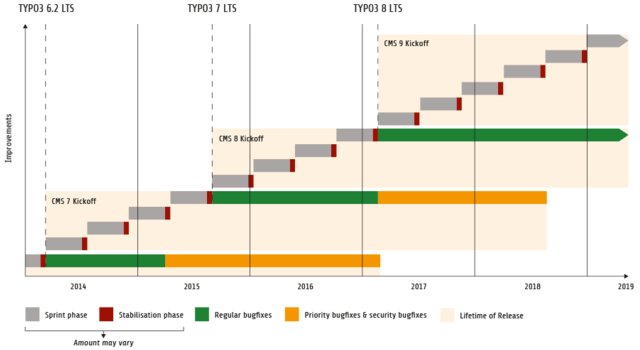
\includegraphics[width=0.90\linewidth]{Introduction/ReleaseAgenda.png}
	\end{figure}

\end{frame}

% ------------------------------------------------------------------------------
% LTXE-SLIDE-START
% LTXE-SLIDE-UID:		2f7c5a1d-ffeeb19d-4019d14a-73280d42
% LTXE-SLIDE-ORIGIN:	83c1fb1c-ed592fa9-a2a279bd-be5cc800 English
% LTXE-SLIDE-ORIGIN:	387f7aeb-53ab533f-95427547-3aa76412 German
% LTXE-SLIDE-TITLE:		TYPO3 CMS Roadmap
% ------------------------------------------------------------------------------
\begin{frame}[fragile]
	\frametitle{Introduction}
	\framesubtitle{Feuille de route TYPO3 CMS}

	Dates de sortie estimées et axes principaux~:

	\begin{itemize}
		\item v7.0 \tabto{1.1cm}02/Déc./2014\tabto{3.4cm}Backend Overhaul Vol 1
		\item v7.1 \tabto{1.1cm}24/Fév./2015\tabto{3.4cm}Core Cleanup \& Streamlining
		\item v7.2 \tabto{1.1cm}28/Avr./2015\tabto{3.4cm}Frontend
		\item v7.3 \tabto{1.1cm}16/Juin/2015\tabto{3.4cm}Package Ecosystem, Composer
		\item v7.4 \tabto{1.1cm}04/Août/2015\tabto{3.4cm}Backend Overhaul Vol 2

		\item
			\begingroup
				\color{typo3orange}
					v7.5 \tabto{1.1cm}29/Sep./2015\tabto{3.4cm}Finalization
			\endgroup

		\item v7 LTS \tabto{1.1cm}Oct./Nov./2015\tabto{3.4cm}\textbf{TYPO3 CMS 7 LTS} (Long Term Release)
	\end{itemize}

	\smaller
		\url{https://typo3.org/typo3-cms/roadmap/}\newline
		\url{http://typo3.org/news/article/embrace-and-innovate-typo3-cms-7/}
	\normalsize

\end{frame}

% ------------------------------------------------------------------------------
% LTXE-SLIDE-START
% LTXE-SLIDE-UID:		499c58b0-f90125ea-8da7c193-d8753c08
% LTXE-SLIDE-ORIGIN:	63decc15-57478e30-70c7ae99-27abd3c2 English
% LTXE-SLIDE-ORIGIN:	3b01edfd-6f06e241-2670b2ad-1b598b4e German
% LTXE-SLIDE-TITLE:		Installation
% ------------------------------------------------------------------------------
\begin{frame}[fragile]
	\frametitle{Introduction}
	\framesubtitle{Installation}

	\begin{itemize}
		\item Procédure officielle d'installation sous Linux/Mac OS X\newline
			(DocumentRoot considéré \texttt{/var/www/site/htdocs})~:
		\begin{lstlisting}
			$ cd /var/www/site
			$ wget --content-disposition get.typo3.org/7.5
			$ tar xzf typo3_src-7.5.0.tar.gz
			$ cd htdocs
			$ ln -s ../typo3_src-7.5.0 typo3_src
			$ ln -s typo3_src/index.php
			$ ln -s typo3_src/typo3
			$ touch FIRST_INSTALL
		\end{lstlisting}

		\item Liens symboliques sous Microsoft Windows~:

			\begin{itemize}
				\item Utiliser \texttt{junction} sous Windows XP/2000
				\item Utiliser \texttt{mklink} sous Windows Vista et Windows 7
			\end{itemize}

	\end{itemize}
\end{frame}

% ------------------------------------------------------------------------------
% LTXE-SLIDE-START
% LTXE-SLIDE-UID:		cba59331-6aa1bb3f-8721385c-d3fe3cd7
% LTXE-SLIDE-ORIGIN:	4dbfb1f2-70930473-ec804474-1c2ac93a English
% LTXE-SLIDE-ORIGIN:	22ce445c-fe028a61-d11c8f8c-510270d3 German
% LTXE-SLIDE-TITLE:		Upgrade to TYPO3 CMS 7
% ------------------------------------------------------------------------------
\begin{frame}[fragile]
	\frametitle{Introduction}
	\framesubtitle{Mise à jour vers TYPO3 CMS 7.x}

	\begin{itemize}
		\item Les mises à jour sont possibles seulement depuis TYPO3 CMS 6.2 LTS
		\item TYPO3 CMS < 6.2 doivent être mis à jour vers la 6.2 LTS en premier
	\end{itemize}

	\begin{itemize}

		\item Instructions de mise à jour~:\newline
			\smaller\url{http://wiki.typo3.org/Upgrade#Upgrading_to_7.5}\normalsize
		\item Guide TYPO3 officiel «~TYPO3 Installation and Upgrading~»~:
			\smaller\url{http://docs.typo3.org/typo3cms/InstallationGuide}\normalsize
		\item De manière générale~:
			\begin{itemize}
				\item Vérifier les prérequis système \small(PHP, MySQL, etc.)
				\item Examiner \textbf{deprecation\_*.log} de l'ancienne instance TYPO3
				\item Mettre à jour toutes les extensions vers leurs dernières versions
				\item Déployer les nouvelles sources et exécuter l'assistant de mise à jour de l'Install Tool
				\item Examiner le module de démarrage des utilisateurs backend (optionnel)
			\end{itemize}
	\end{itemize}

\end{frame}

% ------------------------------------------------------------------------------
